\section{Continous wavelet transformation}

The wavelet transform is used to see the frequency components of the signal in the time frequency domain. Wavelet transformation is practical when looking for signals of lower frequencies compared to the normal fourier analysis, because of the bigger resolution in the wavelet analysis. \cite{Greyer2004} Another drawback of the fourier transform is the loss of time information. 

The wavelet transformation is using a variable sized region windowing technique. Long time intervals are used where low frequency information is computed and short time intervals are used where high frequency information is computed. This is represented in \figref{fig:sigToWave}.

\begin{figure}[H]
	\centering	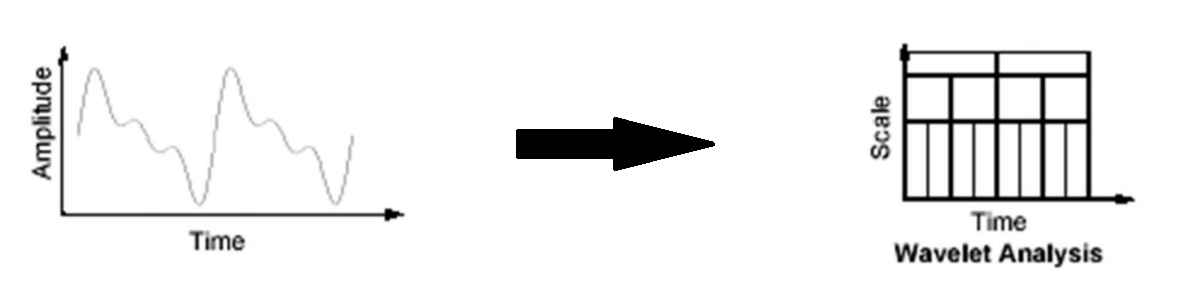
\includegraphics[width=0.65\textwidth]{figures/signalToWavelet}
	\caption{Signal to wavelet computation, modified from \cite{Uvo1995}}
	\label{fig:sigToWave}
\end{figure} \vspace{-.3cm}

The wavelet computes both the scale $(s)$ and position $(p)$ for the wavelet transform. 

\begin{flalign}
	C(s,p)=\int_{-\infty}^{\infty}f(t)\Psi (s,p) dt
	\label{eq:wave}
\end{flalign}

The signal f(t) is convoluted with the wavelet $\Psi$ to get the wavelet coefficients for s and p. 

This is done by computing the wavelet of the signal which then is compared to the wavelet for a section at the beginning of the signal. Then $C$ in equation \ref{eq:wave} is calculated for the section of the signal. The wavelet is shifted to the right and repeated until the entire signal is covered. Then the wavelet is scaled and $C$ is computed for the entire signal again for all scales. \cite{Uvo1995}

Different wavelets can be used to compute the wavelet transformation. In Matlab the default is the Morlet wavelet. 

The general form of the continuous wavelet transform is stated in equation \ref{eq:cwt}:

\begin{flalign}
W(t,s) \equiv \int_{-\infty}^{\infty} \frac{1}{s^n} \psi *(\frac{\tau-t}{\s})x(\tau)d\tau
\label{eq:cwt}
\end{flalign}

Where $\psi *(\frac{\tau-t}{\s})$ is the wavelet and $x(\tau)$ is the signal.\cite{Uvo1995}

The signal or function is put into the continuous wavelet transformation equation \ref{eq:cwt}.
The wavelet transform will give a scolargram as an output.
In Matlab the function cwt can be used to compute the continuous wavelet transformation by inserting the signal and the sampling frequency. This will give a scolargram as shown in \figref{scolargram}. \cite{mathworks2017} 
The frequencies in Hz are shown along the y-axis if the sampling frequency is specified, else it will show the normalized frequency in cycles pr. sample. Along the x-axis is the time vector. The scolargram show the magnitude of the signal to show how the frequency in the signal is distributed. A scale to see the size of the magnitude is also implied. An example of a scolargram is given in \figref{fig:scolargram}

\begin{figure}[H]
	\centering	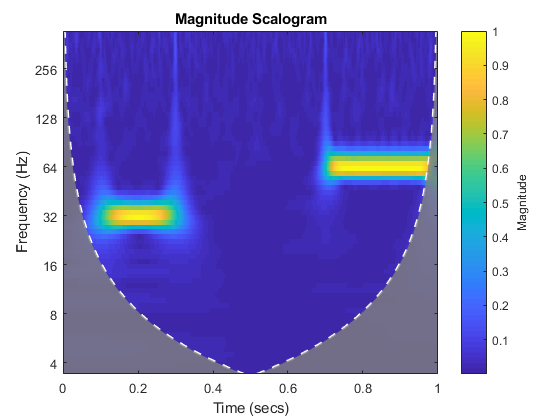
\includegraphics[width=0.65\textwidth]{figures/scolargram}
	\caption{An example of a scolargram, showing frequency content at 32 Hz at time approx 0.2 sec and 64 Hx at approx 0.8 sec \cite{mathworks2017}}
	\label{fig:scolargram}
\end{figure} \vspace{-.3cm}

%\begin{flalign}
%W(t,s) \equiv \int_{-\infty}^{\infty} \frac{1}{s^n} \psi *(\frac{\tau-t}{\s})x(\tau)d\tau
%\label{eq:cwt}
%\end{flalign}

%\begin{flalign}
%	W(t,s) = \frac{1}{2\pi} \int_{-\infty}^{\infty} \Psi*(s\omega)X(\omega)e^{i\omega t} d\omega
%	\label{eq:cwt2}
%\end{flalign}
